
% ----------------------------------------------------------
% Introdução
% ----------------------------------------------------------
\chapter[Introdução]{Introdução}

Dispositivos móveis são amplamente utilizados pelos brasileiros, em 2019 82,7\% dos domicílios brasileiros possuíam acesso à Internet, e 98,6\% deles o faziam através de um telefone celular (IBGE, 2019). Com este alto índice de uso surge também a grande popularidade das redes sociais no país e, por consequência da facilidade de disseminar informação, a necessidade de encontrar lugares confiáveis para se compartilhar e receber informações.

As redes sociais possibilitam a interação de milhões de pessoas, integrando grupos variados de diferentes lugares em um único ambiente virtual. Essas redes funcionam muito bem para lidar com as necessidades de interação da maioria das pessoas, mas não é possível afirmar que se encaixam perfeitamente para todos, afinal, existem públicos que requerem atenção diferenciada, um exemplo deles são as pessoas neurodiversas, que vivenciam uma rotina completamente destoante do convencional.

As barreiras e preconceitos que pessoas neurodivergentes enfrentam na sociedade se iniciam já na dificuldade de acesso à informações corretas e confiáveis sobre o próprio termo que as englobam: neurodiversidade. Um termo designado à condição de pessoas cuja neurobiologia se desenvolveu de forma atípica em relação a um parâmetro médico e biológico que se designa como desenvolvimento normal na espécie humana. O Transtorno de Déficit de atenção (TDAH) e o Transtorno do Espectro Autista (TEA) são exemplos de diagnósticos comuns às pessoas neurodiversas e, apesar de todo o avanço científico dos últimos anos que possibilitam cada vez maior qualidade de vida, existem muitas barreiras de âmbito social que estas pessoas ainda enfrentam. Diante desse cenário, a socialização de milhares de pessoas neurodiversas é prejudicada e, muitas vezes, descredibilizada, e dado que o ser humano é um ser inerentemente social, o que ocorre é que elas têm uma necessidade elementar debilitada e por inúmeras vezes ignorada.

Pela existência das condições ditas é que o diversaGente se mostra um lugar cordial para pais, responsáveis e para as próprias pessoas neurodiversas, com o intuito de tornar-se um local disponível para que todos consigam compartilhar suas experiências, sejam elas experiências ou dicas de vida a serem relatadas por meio do fórum ou experiências vividas em lugares específicos das quais queiram falar sobre e/ou fazer uma avaliação - pontos positivos no atendimento de um restaurante ou profissional de saúde, por exemplo.

\section{Contextualização}

O uso do celular para acessar a internet cresceu significativamente no Brasil. Os aparelhos são o principal meio de acesso à internet, usado pela grande maioria da população brasileira. As informações são da Pesquisa Nacional por Amostra de Domicílios Contínua - Tecnologia da Informação e Comunicação (PNAD Contínua TIC, 2018). Seguindo esse contexto, as redes socias têm ganhado grande relevância nos últimos tempos, modificando significativamente a forma de comunicação e socialização, o ser humano encontrou nos aplicativos de redes sociais uma nova forma de praticar antigos hábitos e atividades que são inerentes aos seres humanos. De acordo com essas circunstâncias, o aplicativo diversaGente é uma rede social com o foco voltado principalmente aos pais de crianças neurodiversas, ou seja, direcionada a um público específico de pessoas. Trazendo consigo a responsabilidade de transmitir maior volume e qualidade de informação sobre este tema, assim como a facilitar a comunicação entre esses pais, mães e responsáveis por essas crianças.

\section{Problematização}

Todo pai, mãe e responsável de uma criança diagnosticada com alguma neurodiversidade compreende e sente a dificuldade de receber esse primeiro diagnóstico. Este momento costuma ser um misto de emoções, terror e medo do que irá acontecer com a criança deste momento em diante. Estes são sentimentos comuns quando se recebem informações desconhecidas até então. No meio em que vivemos, pouco se fala sobre neurodiversidades, mas com um pouco de pesquisa descobrimos que muitas pessoas que apresentam essas condições, podem ter uma vida normal, brincar, estudar, trabalhar e construir relacionamentos, assim como qualquer outra pessoa. A única diferença é que a pessoa diagnosticada com transtorno global de desenvolvimento se desenvolve de forma específica, muitas vezes com uma preocupação a mais em relação ao ambiente e estímulos. Para que seja mais fácil receber esse diagnóstico e para nenhum pai se sentir sozinho estamos criando um aplicativo de rede social voltada para pais e responsáveis de crianças neurodiversas. Para que juntos eles possam compartilhar informações e cuidados, quebrar o preconceito que sentem ao receber o diagnostico, buscar dicas de profissionais especializados em sua região com base em notas e opiniões, atividades úteis para o processo de aprendizado e principalmente entender que não é necessário se esconder, pois agora você faz parte de uma comunidade que te entende e apoia.

\section{Objetivos}

A falta de acesso à informação a respeito do autismo e outros transtornos de desenvolvimento como: Síndrome de Rett, Distúrbio Abrangente do Desenvolvimento , Síndrome de Timothy, Síndrome do X-Frágil, Síndrome de Angelman, Síndrome de Phelan-McDermid, Síndrome de Asperger, TDA: Transtorno do Déficit de Atenção/hiperatividade, entre outras. É um problema que todo pai e mãe nessas condições enfrentam. A diversaGENTE tem como objetivo compartilhar conteúdos de qualidade com facilidade à informação para todos os pais e responsáveis de crianças neurodiversas. Como por exemplo notícias sobre neurodiversidade, boas escolas, médicos ao redor da sua localidade e aspectos de seus filhos divididos pelos pais em grandes fóruns de discussões. Não é uma rede social comum apenas para fazer amigos, é uma comunidade unida para troca de informação e conhecimento.


O aplicativo diversaGente tem como objetivo compartilhar conteúdos de qualidade para todos os pais e responsáveis de crianças neurodiversas. Como, por exemplo, notícias sobre neurodiversidade, boas escolas, médicos próximos a sua localidade e compartilhamento de experiências pelos pais em grandes fóruns de discussões. Não é uma rede social comum apenas para fazer amigos, é uma comunidade unida em prol da troca de informação e conhecimento.

\section{Justificativa}

Um estudo divulgado pela plataforma Cupom Válido, que reuniu dados da Hootsuite e WeAreSocial, mostra que o Brasil é o terceiro país no mundo que usa redes sociais. De acordo com o estudo, os brasileiros ficam, em média 3h42 por dia conectados, ficando atrás somente das Filipinas (4h15) e Colômbia (3h45).
Já em relação as redes sociais, o Brasil conta com mais de 150 milhões de usuários, 70,3\% de sua população. O Sudeste aparece como a região com a maior taxa, cerca de 78\% dos usuários utilizam redes sociais.

Os dados em relação a neurodiversidade ainda não são muito divulgados mas em relação ao autismo podemos destacar que uma em cada 44 crianças aos 8 anos de idade nos Estados Unidos é diagnosticada com o Transtorno do Espectro do Autismo (TEA), segundo relatório do CDC (Centro de Controle de Doenças e Prevenção), (publicado em 2.dez.2021). O número — com dados de 2018 — representa mais um aumento de 22\% em relação ao estudo anterior (1 para 54 — divulgado em 2020). Numa transposição dessa prevalência (de 2,3\% da população) para o Brasil, teríamos hoje cerca de 4,84 milhões de autistas no país. Porém, ainda não temos números de prevalência de autismo no Brasil.

\begin{figure}[htb]
	
	\centering
	\caption{\label{fig_arq_virado}Prevalência de autismo nos EUA 2021}
	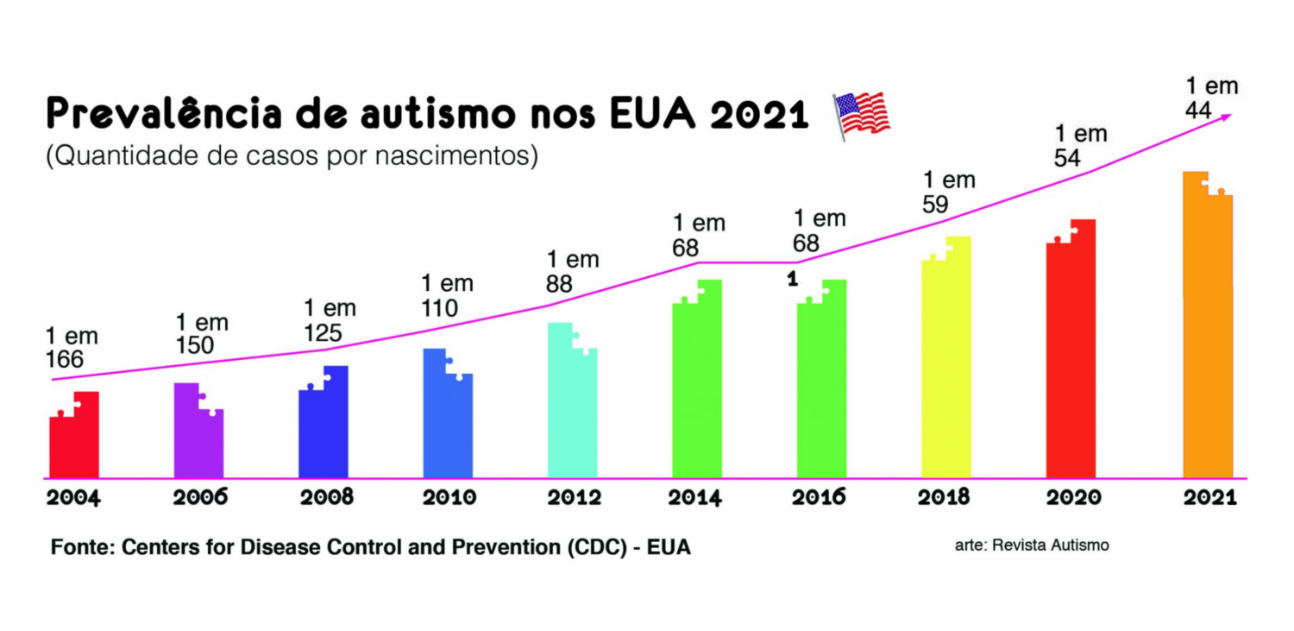
\includegraphics[width=0.9\textwidth]{anexos/diversaGenteGrafico.png}
	\legend{Fonte: Equipe diversaGente}
	\explicacaoErro{A fonte dessa imagem realmente é a gente?}

\end{figure}

Tendo isso em mente, desenvolvemos um aplicativo destinada aos pais e mães de crianças Neurodiversas  pois acreditamos que ter um filho com alguma neurodiversidade traz consigo alguns desafios. Como por exemplo encontrar escolas adequadas e uma lista longa de profissionais especializados. O objetivo do aplicativo é facilitar mesmo que um pouco nesse novo desafio, auxiliar com as escolhas de lugares utilizando notas de profissionais dadas por quem mais entende, os pais e mães. 
Apesar de existirem diversos grupos de discussões sobre neurodiversidades, muitas vezes as informações se perdem ou deixam de serem relevantes. Com nosso aplicativo esse problema não existira mais, terão informações atualizadas e filtros de fácil acesso. Outro ponto importante a ressaltar é que os pais poderão ser agrupados de acordo com o diagnóstico do transtorno global de desenvolvimento do seu filho, favorecendo a troca de informação relevante e mais precisa, facilitando a interação entre famílias. Criando assim uma rede de apoio, não só na escolha de médicos e escolas, mas na troca de informação e cuidados.


\section{Análise de concorrência refinada}

A seção tem o intuito de, através de pesquisas na internet, traçar um comparativo de aplicativos com finalidades similares às do diversaGente e evidenciar as particularidades que esta tem em relação às outras. É possível ver no \autoref{tabela-comparativo} as características de cada aplicação para melhor visualização. 

O primeiro a ser comparado é o Facebook, além de ser uma das redes sociais mais usadas no Brasil e no mundo, possui algumas características similares com o diversaGente, como feed de postagem dentro de grupos, perfil pessoal e opção de compartilhamento de postagens. 

Para o Twitter, uma rede social que é um enorme fórum, muito utilizada entre os jovens, porém não possui nenhuma página para criar grupos e se conversar sobre um assunto específico. Possui um filtro bem eficiente que é possível buscar por algo, caso alguém já tenha feito uma postagem sobre. 

A Tismoo.me é a aplicação mais parecida com o diversaGente, possuindo também um fórum, nichada para o público de pais e responsáveis de crianças pertencentes ao espectro autista. O diversaGente consegue se diferenciar do Tismoo.me pelas funcionalidades de avaliação de locais, sendo possível compartilhar a experiência do usuário e também pela interação de chat em tempo real entre dois usuários. 

A característica principal da Emergency Chat é que pode ser utilizada em qualquer situação onde a fala é impossível, mas a comunicação ainda é necessária. Não é necessariamente uma rede social, possui um chat para comunicação.  

O TippyTalk é um aplicativo voltado para pais ou responsáveis de crianças neurodiversas, principalmente aquelas com alguma dificuldade de comunicação verbal. Permite que um administrador crie imagens exclusivamente identificáveis e familiares para as crianças, apoiando na educação e treino de atividades/tarefas rotineiras. 

O The Autism Helper também tem grande similaridade com o diversaGente porque é voltado para quem procura a facilitar, o máximo possível, a vida de indivíduos do espectro autista. O aplicativo possui fóruns para discussão e perfil pessoal. 


\begin{quadro}[thb]
	\centering
	\ABNTEXfontereduzida
	\caption[Comparativo entre aplicações]{Comparativo entre aplicações}
	\label{tabela-comparativo}

	\begin{tabular}{|l|c|c|c|c|c|c|c|}
		\hline
		\thead{ } & \thead{diversa\\Gente} & \thead{Facebook}  & \thead{Twitter}  & \thead{Tismoo\\.me} & \thead{Emergency\\ Chat}  & \thead{Tippy\\ Talk}  & \thead{The \\Autism \\Helper}\\
		\hline
		Público Neurodiverso & X &  &  & X & X & X & X \\
		\hline
		Consultar Notícias & X &  & X & X &  &  &  \\
		\hline
		Fóruns & X & X &  & X &  &  & X \\
		\hline
		Locais Avaliados & X &  &  &  &  &  & \\
		\hline
		Chat & X & X & X &  & X & X &  \\
		\hline
		Feed de Postagem & X & X & X & X &  &  & X\\
		\hline
		Perfil Pessoal & X & X & X & X &  &  & \\
		\hline
		Buscar Usuários & X & X & X & X &  &  & \\
		\hline
		Compartilhar & X & X & X & X &  &  & X \\
		\hline
	\end{tabular}
\fonte{Equipe diversaGente (2022)}
\end{quadro}



